\documentclass[aspectratio=169]{beamer}

% =============================================================
% PREAMBLE
% =============================================================

% --- PACKAGES ---
\usepackage[english]{babel}
\usepackage[T1]{fontenc}
\usepackage[utf8]{inputenc} 
\usepackage{graphicx}
\usepackage{booktabs} % For professional tables
\usepackage{tikz}     % For the pipeline diagram
\usetikzlibrary{calc, positioning, arrows}
\usetikzlibrary{shapes.geometric, arrows, positioning}
\usepackage{hyperref}
\usepackage{colortbl}
% --- CUSTOM BEAMER STYLE CONFIGURATION ---
% These must be defined BEFORE loading custom_beamer.sty

\def\true{1}
\def\false{2}

\def\colortheme{dark} % preset themes available are lighten, light, dark
\def\alertcolor{dark} % preset themes available are lighten, light, dark
\def\upperbar{\true} % i want upper index/navigation bar, \true or \false
\def\bottomsectionbar{\true} % i want bottom bar with Title and Frame/Slide number, \true or \false
\def\bottomtitlebar{\true} % i want bottom bar with Section and Institute, \true or \false

% Fix for alertblock colors
\usecolortheme{default}

% --- LOAD YOUR UNIVERSITY STYLE ---
\usepackage{custom_beamer}

% --- BIBLIOGRAPHY CONFIGURATION ---
\usepackage[style=authoryear, backend=biber]{biblatex} % Author-Year style
\addbibresource{references.bib} % Loads the file created above
%\renewcommand*{\bibfont}{\footnotesize} % Makes the font smaller to fit the slide


% % %
\if\upperbar\false
    \setbeamertemplate{headline}{}
\fi
% % %

% --- METADATA ---
\title[Dense vs. Sparse Retrieval]{Reproducing ``Experimental Analysis of Dense vs.~Sparse Retrieval''}
% \subtitle{An Experimental Analysis of Dense vs. Sparse Retrieval on the BEIR Benchmark}
\author{Gabriele Righi}
\institute{University of Pisa}
\date{\today}

% Repository link in the footer or title
\newcommand{\repoLink}{\url{https://github.com/Gheb6/dense-vs-sparse-retrieval}}

\begin{document}

% =============================================================
% SLIDE 1: Title Slide
% =============================================================
\firstpage

% =============================================================
% SLIDE 2: Introduction & Motivation
% =============================================================
\section{Introduction}

\begin{frame}{Introduction \& Research Goals}
    \textbf{Context: The ``Operational'' Gap}
    \begin{itemize}
        \item Modern IR has shifted from Sparse (BM25) to Dense (Embeddings).
        \item Dense retrieval is effective but resource-intensive.
    \end{itemize}
    
    \vspace{0.5em}
    
    \begin{alertblock}{The 3 Research Questions (Lin et al., 2024)}
        This project reproduces the analysis to answer three key operational questions:
        \begin{enumerate}
            \item \textbf{RQ1:} Is the complexity of HNSW always necessary, or is \textbf{Flat index} sufficient for typical workloads?
            \item \textbf{RQ2:} Can we use \textbf{INT8 Quantization} to save RAM without hurting retrieval quality (nDCG)?
            \item \textbf{RQ3:} How does \textbf{Sparse Retrieval} (BM25/SPLADE) compare to Dense methods in a modern GPU environment?
        \end{enumerate}
    \end{alertblock}
\end{frame}
% =============================================================
% SLIDE 3: Experimental Setup
% =============================================================
\section{Experimental Setup}

\begin{frame}{Experimental Setup}
    \begin{itemize}
        \item \textbf{Benchmark}: BEIR (Heterogeneous Evaluation).
        \item \textbf{Datasets Analyzed}: \texttt{scifact}, \texttt{nfcorpus}, \texttt{cqadupstack} (Android, Gaming, GIS).
        \item \textbf{Hardware}: NVIDIA T4 GPU (16GB VRAM).
        \begin{itemize}
            \item \textit{Constraints simulated a realistic production environment.}
        \end{itemize}
    \end{itemize}

    \vspace{1em}
    \textbf{Metrics}
    \begin{description}
        \item[nDCG@10] Retrieval Quality (Ranking accuracy).
        \item[Recall@10] Retrieval Coverage (Relevant items found).
        \item[QPS] Queries Per Second (Throughput/Speed).
    \end{description}
\end{frame}


% =============================================================
% --- NEW SLIDE 4: CHALLENGE 1 (Pyserini vs Faiss) ---
% =============================================================

\begin{frame}{Challenge I: The Missing Link in Pyserini}
    \textbf{Original Plan}: Use \texttt{Pyserini} (Lucene wrapper) for \textit{both} Sparse (BM25) and Dense (HNSW) indexing, matching the paper exactly.
    
    \vspace{1em}
    \textbf{The Obstacle}:
    \begin{itemize}
        \item Pyserini supports HNSW via Java, but the **Python API for adding vectors to HNSW indexes is limited/missing**.
        \item Impossible to feed custom BGE embeddings directly into Pyserini's HNSW from Python easily.
    \end{itemize}
    
    \vspace{1em}
    \textbf{The Engineering Pivot: Hybrid Pipeline}
    \begin{itemize}
        \item \textbf{Sparse Path:} Retained Pyserini for BM25 (Industry Standard).
        \item \textbf{Dense Path:} Migrated to \textbf{Faiss} (Facebook AI Similarity Search).
        \item \textit{Why?} Faiss offers native \textbf{GPU support} and flexible python bindings for custom embeddings, enabling a fairer comparison for RQ1 (Flat vs HNSW).
    \end{itemize}
\end{frame}

% =============================================================
% SLIDE 5: The SPLADE Anomaly (The Problem)
% =============================================================
\begin{frame}{Challenge II: The SPLADE Underperformance Mystery}
    \textbf{The Anomaly}
    While BM25 and Dense Retrieval matched the paper's baselines immediately, the standard SPLADE implementation (via Pyserini) failed.

    \begin{table}
        \centering
        \small
        \begin{tabular}{llcc}
            \toprule
            \textbf{Method} & \textbf{Implementation} & \textbf{nDCG@10} & \textbf{Status} \\
            \midrule
            BM25 & Pyserini (Lucene) & 0.323 & \textcolor{green!60!black}{\textbf{Success}} \\
            BGE Dense & Faiss & 0.370 & \textcolor{green!60!black}{\textbf{Success}} \\
            \textbf{SPLADE} & \textbf{Pyserini Impact} & \textbf{0.230} & \textcolor{red}{\textbf{Fail (-28\%)}} \\
            \bottomrule
        \end{tabular}
    \end{table}

    \vspace{0.5em}
    \textbf{Root Cause Analysis}
    \begin{itemize}
        \item \textit{Hypothesis A (Wrong Model)}: Switched to \texttt{selfdistil}. No change.
        \item \textit{Hypothesis B (Quantization)}: Forced integer scaling ($w \times 100$). No change.
        \item \textbf{Conclusion}: Pyserini's ``Black Box'' Impact Indexing was introducing \textbf{lossy compression artifacts}, destroying the precision of sparse weights.
    \end{itemize}
\end{frame}

% =============================================================
% SLIDE 6: The Solution (Matrix Engine) - CONDENSED
% =============================================================
\begin{frame}{The Solution: Custom Matrix Engine}
    \textbf{The Fix}: Bypassed Pyserini. Built a \textbf{pure Python sparse engine} using \texttt{SciPy}.

    \vspace{1em}

    \begin{columns}
        \column{0.55\textwidth}
        \textbf{Methodology}
        \begin{itemize}
            \item \textbf{Direct Encoding}: Used HuggingFace to avoid quantization artifacts.
            \item \textbf{Vectorized Search}: Replaced index lookup with Matrix Multiplication.
        \end{itemize}
        
        \column{0.4\textwidth}
        \begin{block}{Core Logic}
            \centering
            \[ S = \mathbf{D} \times \mathbf{q}^T \]
        \end{block}
    \end{columns}

    \vspace{1em}

    \begin{alertblock}{Impact}
        \begin{itemize}
            \item \textbf{Quality}: nDCG@10 restored to $\mathbf{0.357}$ (vs 0.230).
            \item \textbf{Speed}: $\sim$296 QPS (Efficient on Python).
        \end{itemize}
    \end{alertblock}
\end{frame}



% =============================================================
% SLIDE 7: Implementation Pipeline (FIXED GEOMETRY)
% =============================================================
\section{Implementation}

\begin{frame}{Implementation Pipeline: The ``Dual-Engine'' Architecture}
    \begin{center}
    \resizebox{1.0\textwidth}{!}{
        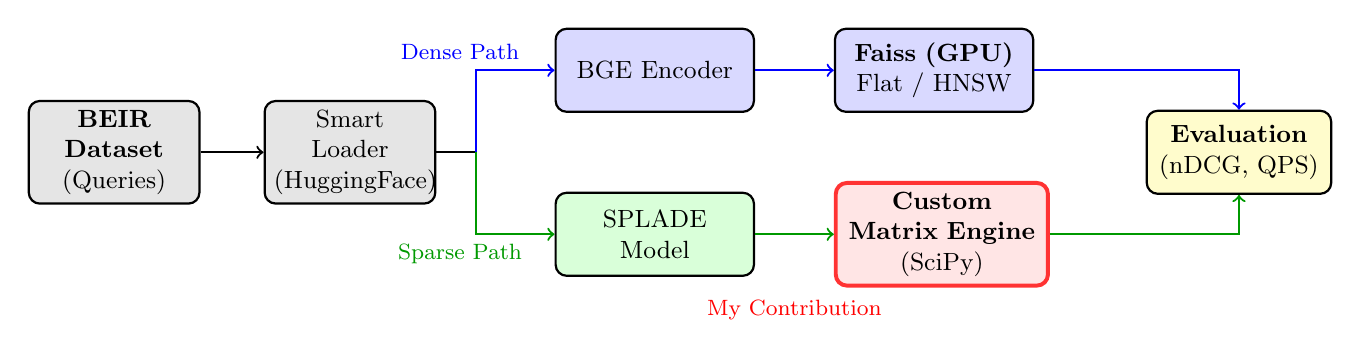
\begin{tikzpicture}[
            node distance=1.0cm, 
            auto,
            base/.style = {rectangle, draw=black, thick, text centered, rounded corners, minimum height=3em, font=\small},
            data/.style = {base, fill=gray!20, text width=5.5em},
            dense/.style = {base, fill=blue!15, text width=6.5em},
            sparse/.style = {base, fill=green!15, text width=6.5em},
            custom/.style = {base, draw=red!80, fill=red!10, text width=7em, line width=0.5mm}, 
            eval/.style = {base, fill=yellow!20, text width=6em}
        ]

            % --- 1. Nodes ---
            \node [data] (dataset) {\textbf{BEIR Dataset} \\ (Queries)};
            \node [data, right=0.8cm of dataset] (loader) {Smart Loader \\ (HuggingFace)};
            \node [coordinate, right=0.5cm of loader] (split) {};

            \node [dense, above right=0.5cm and 1cm of split] (bge) {BGE Encoder};
            \node [dense, right=1cm of bge] (faiss) {\textbf{Faiss (GPU)} \\ Flat / HNSW};

            \node [sparse, below right=0.5cm and 1cm of split] (splade) {SPLADE Model};
            \node [custom, right=1cm of splade] (matrix) {\textbf{Custom Matrix Engine} \\ (SciPy)};

            % Position Evaluation centered
            \node [eval] (eval) at ($(faiss.east)!0.5!(matrix.east) + (2.5, 0)$) {\textbf{Evaluation} \\ (nDCG, QPS)};

            % --- 2. Connections with FIXED LABELS ---
            
            % Input
            \draw [->, thick] (dataset) -- (loader);
            \draw [-, thick] (loader) -- (split);

            % Dense Path (Blue)
            % xshift=-0.5cm moves the text to the left to avoid touching the BGE box
            \draw [->, thick, blue] (split) |- node[pos=0.8, above, xshift=-0.8cm, font=\footnotesize] {Dense Path} (bge);
            \draw [->, thick, blue] (bge) -- (faiss);
            \draw [->, thick, blue] (faiss.east) -| (eval.north); 

            % Sparse Path (Green)
            % xshift=-0.5cm moves the text to the left to avoid touching the SPLADE box
            \draw [->, thick, green!60!black] (split) |- node[pos=0.8, below, xshift=-0.8cm, font=\footnotesize] {Sparse Path} (splade);
            
            % My Contribution
            % yshift=-3pt lowers the text to detach it from the line (updated to 20pt in code)
            \draw [->, thick, green!60!black] (splade) -- node[midway, below=20pt, red, font=\footnotesize] {My Contribution} (matrix);
            
            \draw [->, thick, green!60!black] (matrix.east) -| (eval.south);

        \end{tikzpicture}
    }
    \end{center}

    \vspace{0.5em}
    \textbf{Architectural Highlights:}
    \begin{itemize}
        \item \textbf{Parallel Processing:} Simultaneous execution of Dense and Sparse pipelines.
        \item \textbf{\textcolor{red}{Custom Matrix Engine}}: Replaced Pyserini's ``Black Box'' indexer with a transparent vector-matrix multiplication engine for SPLADE.
        \item \textbf{GPU Acceleration}: Integrated Faiss to unlock GPU speeds for Dense Retrieval.
    \end{itemize}
\end{frame}

%%%%%%%%%%%%%%%%%%%%%%%%%%%%%%%%%%%%%%%%%%%%%%%%%
%%%%%%%%%%%%%%%%%%%%%%%%%%%%%%%%%%%%%%%%%%%%%%%%%
%%%%%%%%%%%%%%%%%%%%%%%%%%%%%%%%%%%%%%%%%%%%%%%%%
\section{Results: Quality}

\begin{frame}{Operational Advice: RQ1 \& RQ2}

    % Titolo leggermente più piccolo per guadagnare spazio
    \small \textbf{Summary: When to switch Index? When to Quantize?}
    \vspace{0.1em}

    \begin{table}
        \centering
        \scriptsize % Carattere piccolo ma leggibile
        \setlength{\tabcolsep}{3pt} % Riduce spazio tra colonne
        \renewcommand{\arraystretch}{1.1} % Riduce altezza righe
        \begin{tabular}{l l c c c l}
            \toprule
            \textbf{Dataset} & \textbf{Method} & \textbf{Build} & \textbf{RAM} & \textbf{QPS} & \textbf{Verdict / Trade-off} \\
            \midrule
            
            % SCIFACT
            \textbf{SciFact} 
            & Flat (FP32) & \textbf{$<$0.1s} & .01 GB & \textbf{4,205} & \textcolor{green!60!black}{\textbf{Best Choice}} \\
            \textit{(5k)}
            & Flat (INT8) & $<$0.1s & .01 GB & 2,209 & \textcolor{red!80!black}{\textit{Slower (CPU limit)}} \\
            \cmidrule(l){2-6}
            
            % QUORA
            \textbf{Quora} 
            & Flat (FP32) & \textbf{1s} & .38 GB & 120 & \textit{Too Slow} \\
            \textit{(523k)}
            & HNSW (FP32) & 234s & .45 GB & \textbf{361} & \textcolor{blue}{\textbf{Worth Build Cost}} \\
            \cmidrule(l){2-6}
            
            % NQ
            \textbf{NQ} 
            & HNSW (FP32) & 25m & 2.4 GB & 9,034 & \textit{High RAM} \\
            \textit{(2.6M)}
            & HNSW (\textbf{INT8}) & 25m & \textbf{0.6 GB} & \textbf{9,100} & \textcolor{blue}{\textbf{-75\% RAM (Safe)}} \\
            
            \bottomrule
        \end{tabular}
    \end{table}

    \vspace{-0.5em}

    % Un unico blocco per risparmiare spazio verticale
    \begin{block}
        \scriptsize % Testo piccolo nel blocco
        \begin{itemize}
            \setlength\itemsep{0.2em} % Riduce spazio tra i punti
            \item \textbf{RQ1 (Scale):} Use \textbf{Flat} for small data ($<$100k) due to zero build time. Use \textbf{HNSW} for large data ($>$200k) where Flat search becomes too slow.
            \item \textbf{RQ2 (Quantization):} 
            \begin{itemize}
                \item \textbf{HNSW:} Always use INT8. It saves 75\% RAM with $<1\%$ quality loss.
            \end{itemize}
        \end{itemize}
    \end{block}

\end{frame}

% =============================================================
% SLIDE 9: Quality Analysis (FINAL WITH SETUP COST)
% =============================================================


\begin{frame}{Quality Analysis: Sparse vs. Learned Sparse vs. Dense}
    
    \textbf{Q: Does SPLADE bridge the gap? Is Dense still superior?}

    \vspace{-0.5em}

    \begin{table}
        \centering
        \footnotesize 
        \setlength{\tabcolsep}{5pt}
        \begin{tabular}{l c c c c}
            \toprule
            \textbf{Dataset} & \textbf{BM25} & \textbf{SPLADE} & \textbf{Dense} & \textbf{Winner} \\
            \midrule
            \textbf{SciFact} & 0.679 & 0.717 & \textbf{0.738} & \textcolor{blue}{\textbf{Dense}} \\
            \textit{(Small)} & & & \textit{(Flat FP32)} & \\
            \midrule
            \textbf{Quora} & 0.789 & 0.842 & \textbf{0.889} & \textcolor{blue}{\textbf{Dense}} \\
            \textit{(Medium)} & & & \textit{(Flat FP32)} & \\
            \midrule
            \textbf{NQ} & 0.235 & \textbf{0.577}* & \textbf{0.541} & \textcolor{blue}{\textbf{Dense}} \\
            \textit{(Large)} & & \textit{(Subset 100k)} & \textit{(Flat FP32)} \\
            \bottomrule
        \end{tabular}
    \end{table}

    \vspace{-0.5em}
    
    \begin{block}{}
        \footnotesize
        \begin{itemize}
            \setlength\itemsep{0.2em}
            \item \textbf{Small/Medium Data:} SPLADE improves over BM25 significantly (+15-20\%).
            \item \textbf{NQ Result:} Dense is the winner, but required \textbf{$\sim$4h GPU encoding} (vs BM25 minutes).
            \item \textbf{*Note on SPLADE:} Due to computational constraints, SPLADE was evaluated on a \textbf{100k subset}. 
            \item \textbf{Conclusion:} Dense Retrieval provides the best quality, justifying the high setup cost.
        \end{itemize}
    \end{block}
\end{frame}

% =============================================================
% SLIDE 10: Conclusions
% =============================================================
\section{Conclusions}

\begin{frame}{Conclusions \& Operational Advice}
    \textbf{Answering the Research Questions:}
    
    \vspace{0.5em}
    
    \begin{itemize}
        \item[\textbf{RQ1}] \textbf{HNSW vs Flat:} 
        \textit{Verdict:} HNSW is \textbf{not} always necessary. \textbf{Flat Index} is faster for datasets $<100$k docs and simpler to maintain.
        
        \item[\textbf{RQ2}] \textbf{Quantization Safety:} 
        \textit{Verdict:} \textbf{Yes.} INT8 reduces RAM by 75\% with negligible quality loss ($<1\%$ nDCG drop). It should be the default.
        
        \item[\textbf{RQ3}] \textbf{Sparse vs Dense:} 
        \textit{Verdict:} Dense methods (BGE) generally outperform Sparse (BM25) in quality, but custom Sparse implementations (Matrix Engine) can be extremely fast on GPU.
    \end{itemize}
    
    \vspace{1em}
    
    \begin{block}{Final Recommendation}
        For most production scenarios under 1M docs: \textbf{Use Dense Retrieval with Flat Index + INT8 Quantization.}
    \end{block}
\end{frame}


% =============================================================
% SLIDE 11: References
% =============================================================
\begin{frame}[allowframebreaks]{References}
    \nocite{*} % Prints ALL references from the .bib file
    \printbibliography
\end{frame}

% =============================================================
% SLIDE 12: Q&A
% =============================================================
\begin{frame}
    \centering
    \Huge \textbf{Thank you!}
    
    \vspace{1em}
    \Large Questions?
    
    % \vspace{2em}
    % \normalsize
    % \repoLink
\end{frame}

\end{document}